\begin{figure}
    \centering
    \subfigure[{$\scriptstyle h^\star(\vec x) = x_1+x_1x_2$}]{%
        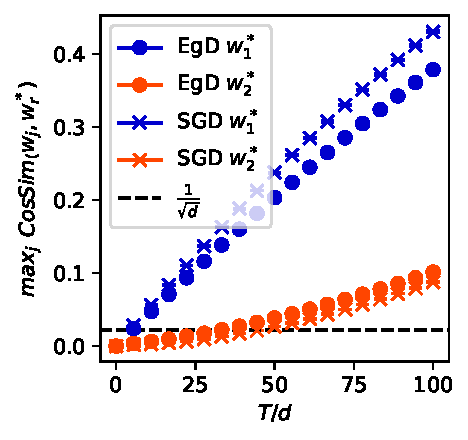
\includegraphics[height=0.22\textwidth, trim={0 8 0 0}, clip]{figs/fig2_k1_kstar1}
        \label{2405:fig:multi_index_1}
    }
    \subfigure[{$\scriptstyle h^\star(\vec x) = \mathrm{sign}{(x_1x_2)}$}]{%
        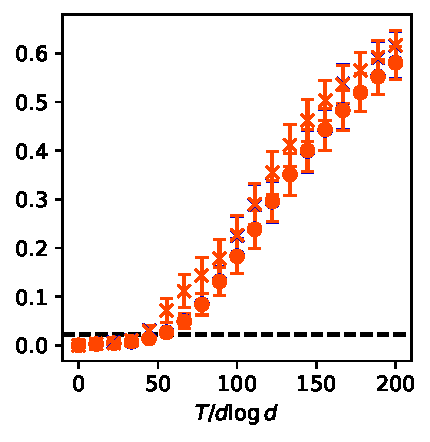
\includegraphics[height=0.22\textwidth, trim={0 8 0 0}, clip]{figs/fig2_k2_kstar2}
        \label{2405:fig:multi_index_2}
    }
    \subfigure[{$\scriptstyle h^\star(\vec x) = x_1+\mathrm{He}_3(x_2)$}]{%
        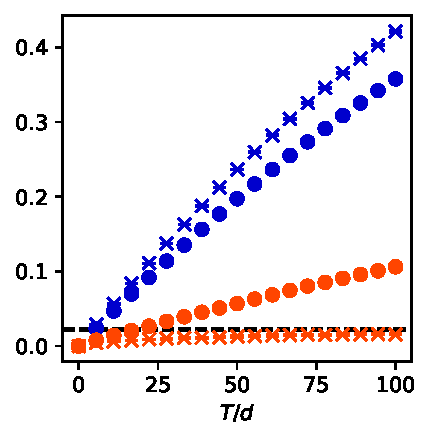
\includegraphics[height=0.22\textwidth, trim={0 8 0 0}, clip]{figs/fig2_k3_kstar1}
        \label{2405:fig:multi_index_3}
    }
    \subfigure[{$\scriptstyle h^\star (\vec x) = x_1x_2x_3$}]{%
        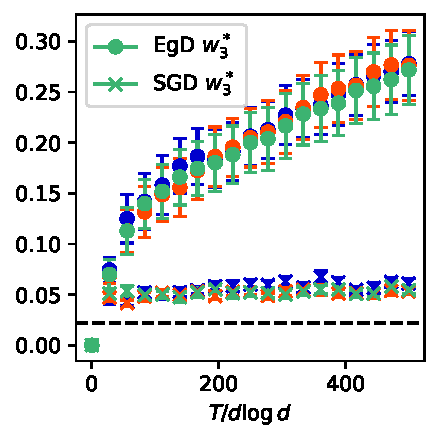
\includegraphics[height=0.22\textwidth, trim={0 8 0 0}, clip]{figs/fig2_k3_kstar2}
        \label{2405:fig:multi_index_4}
    }

    \caption{\textbf{Learning multi-index targets --}
    Evolution of the maximum Cosine Similarities attained by EgD (crosses) and SGD (dots) as a function of the normalized iteration time. The Different directions $\{\vec w^\star_r\}_{r \in [k]}$ are identified by colors: $\vec w^\star_1$ (blue), $\vec w^\star_2$ (orange), $\vec w^\star_3$ (green).
     (dashed horizontal line $\frac{1}{\sqrt{d}}$ is a visual guide to place random performance). 
    \textbf{(a)~$(\ell,\ell^\star)=(1,1)$:} both  algorithms learn the first direction in linear time, as well the second one in $O(d)$ steps using the staircase mechanism.
    \textbf{(b) $(\ell,\ell^\star)=(2,2)$:} both  algorithms learn the two directions simultaneously in $O(d\log d)$ steps.
    \textbf{(c)~$(\ell_{\vec w^\star_2},\ell_{\vec w^\star_2}^\star)=(3,1)$:} both algorithms learn $\vec w^\star_1$ in linear time, but only EgD learns $\vec w^\star_2$ in $O(d)$; SGD instead requires $O(d^2)$.
    \textbf{(d) $(\ell,\ell^\star)=(3,2)$:} EgD learns all 3 directions simultaneously in $O(d\log d)$ steps, while SGD needs $O(d^2)$ time.  (Details in App.~\ref{2405:sec:app:implementation}).}
    \label{2405:fig:main:multi_index_complete}
\end{figure}

\section{Multi-Index Model}
We now investigate the superiority of Algorithm~\ref{2405:algo:optimizer_main_step} over the idealized One-Pass SGD training scheme when learning multi-index targets. In this setting, the networks weights can align with only a few select directions from $V^\star$. To quantify this behavior, we define directional versions of the Information and Generative Exponents (see also \citep{troiani2024fundamental}):
\begin{definition}\label{2405:def:ie_pge_multi}
    Let $\vec{v}\in V^\star$. The Information Exponent $\ell_{\vec{v}}$ (resp. Polynomial Generative Exponent $\ell^\star_{\vec{v}}$) of $y$ in the direction $\vec v$ is the smallest $k$ such that
    \[ \Ea{yH_k(\langle \vec{v}, \vec{z} \rangle)} \neq 0 \quad (\text{resp.} \  \Ea{p_{\vec{v}}(y)H_k(\langle \vec{v}, \vec{z} \rangle)} \neq 0 ) \]
    for a polynomial $p_{\vec{v}}$. We also let $\ell = \min_{\vec{v}}\ell_{\vec{v}}$ and $\ell_p^\star = \min_{\vec{v}}\ell^\star_{\vec{v}}$.  The minimal subspace $U^\star \subseteq V^\star$ is defined as the smallest subspace $U$ such that $\ell_\vec{v} > \ell$ (resp. $\ell_{\vec{v}}^\star > \ell_p^\star$) for every $v\in U^\bot$.
\end{definition}
The identification of the class of hard functions has been subject of intense theoretical scrutiny \citep{abbe2021staircase,abbe2022merged,abbe2023sgd,dandi2023how,bietti2023learning,troiani2024fundamental}; and for the problem of initial alignment it was shown to depend on the Information exponent defined above. 
Thus, similarly to the single-index scenario, the time complexity needed for Algorithm~\ref{2405:algo:optimizer_main_step} to weakly recover the target subspace follows the law in eq.~\eqref{2405:eq:gba_time_scaling} for the multi-index information exponent $\ell$. A natural question is thus to ask whether the class of Algorithm~\ref{2405:algo:optimizer_main_step} also allows us to bypass this requirement. We show that this is indeed the case. Consider a neural network as in Equation~\eqref{2405:eq:def_nn}; we assume that the internal learning rate $\rho$ is chosen independently for each neuron:
\begin{assumption}
    For each $j \in [p]$, the parameter $\rho_{0, j}$ is chosen independently from all other neurons, according to a \emph{symmetric} distribution which is absolutely continuous w.r.t the Lebesgue measure.
\end{assumption}

\begin{theorem}\label{2405:thm:multi_index_recovery}
    Let $\delta > 0$, and $\Pi^\star$ the projection operator on $V^\star$. There exists constants $\gamma_0(\delta), C(\delta)$ depending only on $\delta$ such that if we take $p \geq C(\delta)k$ and
    \begin{itemize}
        \item if $\ell_p^\star = 1$, $\gamma = \gamma_0(\delta) d^{-1}$ and $T = C(\delta)d$,
        \item if $\ell_p^\star = 2$, $\gamma = \gamma_0(\delta) (d\log(d))^{-1}$ and $T = C(\delta)d\log(d)^2$,
    \end{itemize}
    then with probability $1 - \delta$, there exists a $t \leq T$ such that at least a positive proportion of the vectors $\vec{w}_{t, i}$ satisfy $\norm{\Pi^\star \vec{w}_{t, i}} \geq \eta$.
Further, if $\ell_p^\star = 1$, then the vectors $\{\Pi^\star \vec{w}_{t, i}\}_{i \in [p]}$ span the minimal subspace $U^\star$.
\end{theorem}

\begin{figure}
    \centering
    \subfigure[ ${\scriptstyle h^\star(\vec x)= x_1 + x_1 \mathrm{He}_3(x_2)}$]{%
        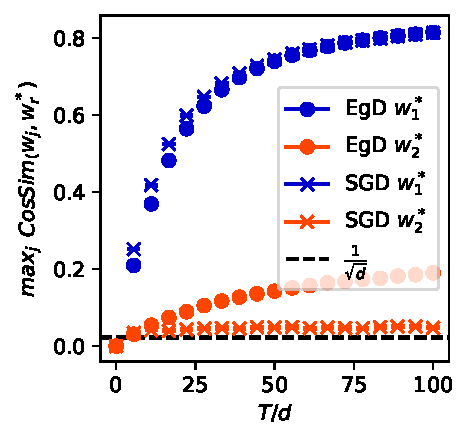
\includegraphics[height=0.23\textwidth, trim={0 8 0 0}, clip]{figs/fig2_k3_kstar1_staircase}
        \label{2405:fig:staircase_1}
    }
     \subfigure[${\scriptstyle h_{\mathrm{sign}}^\star(\vec{x}) = \mathrm{sign}(x_1x_2x_3), \quad h^\star_{\mathrm{stair}}(\vec x) = \mathrm{He}_2(x_1) + \mathrm{sign}(x_1x_2x_3)}$]{%
        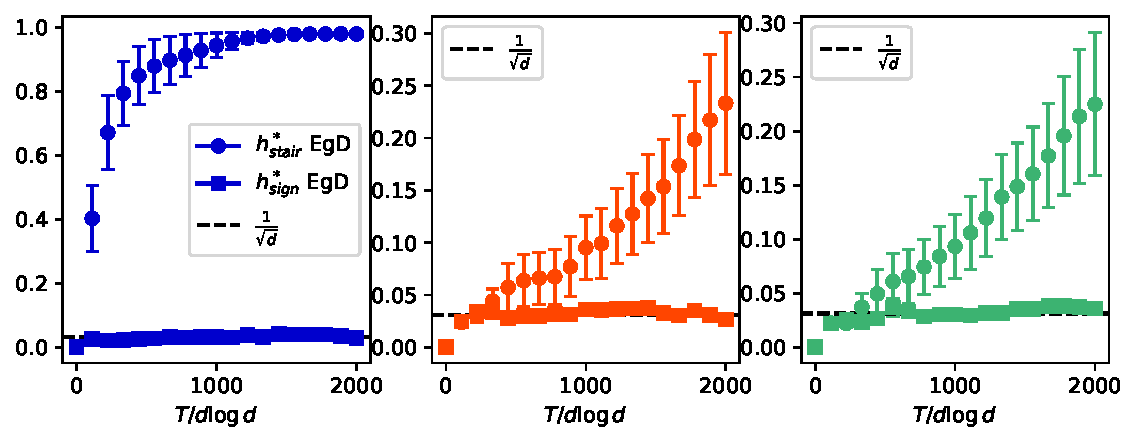
\includegraphics[height=0.23\textwidth, trim={0 8 0 0}, clip]{figs/figs_SQStair_long}
        \label{2405:fig:staircase_2}
    }
    \caption{\textbf{Hierarchical learning --} Evolution of the maximum Cosine Similarities with different target directions $\{\vec w^\star_r\}_{r \in [k]}$ are identified by different colors: $\vec w^\star_1$ (blue), $\vec w^\star_2$ (orange), $\vec w^\star_3$ (green) as a function of the normalized iteration time.
    \textbf{(a):} both the algorithms learn $\vec w^\star_1$ in linear time, but only EgD can also learn $\vec w^\star_2$ in $O(d)$ via a staircase mechanism; SGD requires another $O(d^2)$ steps to take advantage of the staircase and learn $\vec w^\star_2$.
    \textbf{(b):} EgD performance for the target function $f^\star_{\mathrm{stair}}$ (dots) and $f^\star_{\mathrm{sign}}$(squares); we plot in separate subplots the overlap with different directions to highlight the presence of hierarchical learning mechanism. Learning the first target direction $\vec w^\star_1$ triggers the hierarchical mechanism and EgD is able to weakly recover the full target subspace $\mathrm{Span}(\vec w^\star_1, \vec w^\star_2, \vec w^\star_3)$ in $O(d \log d)$, while this does not happen when removing $\mathrm{He}_2(x_1)$ from the target.
    See App.~\ref{2405:sec:app:implementation} for additional details.}
    \label{2405:fig:main:staircase1}
\end{figure}

\subsection{Numerical investigation with multi-index target}\label{2405:subsec:multi_numerics}

% (\lp{Def.~\ref{2405:def:hardness_subspace}}). 
We illustrate the results of Thm.~\ref{2405:thm:multi_index_recovery} numerically by comparing the performance of One-Pass SGD with Alg.~\ref{2405:algo:optimizer_main_step} in Fig~\ref{2405:fig:main:multi_index_complete}. We measure the maximal cosine similarity between the hidden layer neurons and the different rows of the target's weight matrix $W^\star$ as a function of the iteration time. We set without loss of generality the target's directions to the standard basis of $\mathbb{R}^d$ to ease the notation. The algorithms considered are again EgD and vanilla One-Pass SGD (See App.~\ref{2405:sec:app:implementation} for details).
\begin{itemize}
\item \textbf{SGD-easy non-symmetric targets ($\ell = \ell^\star = 1$) --} Fig.~\ref{2405:fig:main:multi_index_complete}, left, shows $h^\star(x_1,x_2) = x_1 + x_1x_2$. Here both SGD and Alg.~\ref{2405:algo:optimizer_main_step} learn in $T= O(d)$ the directions $(\vec w^\star_1, \vec w^\star_2)$.

\item \textbf{SGD-easy symmetric targets ($\ell = \ell^\star = 2$) --} Fig.~\ref{2405:fig:main:multi_index_complete}, center left, shows $h^\star(x_1,x_2) = x_1x_2$.  Here both SGD and Alg.~\ref{2405:algo:optimizer_main_step} learn in $T=O(d \log d)$ the directions $(\vec w^\star_1, \vec w^\star_2)$. 

\item \textbf{Non-symmetric targets with SGD-easy and hard directions ($\ell_{\vec{v}} > 2, \ell^\star_{\vec{v}}=1$) --} Fig.~\ref{2405:fig:main:multi_index_complete}, center-right, shows $h^\star(x_1,x_2) = x_1 + \mathrm{He}_3(x_2) $. Here both SGD and Alg.~\ref{2405:algo:optimizer_main_step} learn in $T=O(d)$ the direction $\vec w^\star_1$, that satisfies $\ell_{\vec{w_1^\star}} = \ell_{\vec{w_1}^\star}^\star = 1$. However, since $\ell_{\vec{w_2^\star}} = 3$ while $\ell_{\vec{w_2^\star}}^\star = 1$, One-Pass SGD suffers from the limitations detailed in eq.~\eqref{2405:eq:gba_time_scaling} and requires $\Omega(d^2)$ samples to learn the second direction $\vec w^\star_2$. This contrasts with the behaviour of Alg.~\ref{2405:algo:optimizer_main_step} that learns also $\vec w^\star_2$ in $T=O(d)$ steps.

\item \textbf{SGD-hard symmetric targets ($\ell > 2,  \ell^\star =2$) --} The right section Fig.~\ref{2405:fig:main:multi_index_complete} shows $h^\star(x_1,x_2,x_3) = x_1 x_2 x_3$. The Information Exponent is $\ell=3$, hence vanilla SGD does not learn any direction in the target subspace in $T=O(d \log d)$ iterations. However, Algorithms~\ref{2405:algo:optimizer_main_step} learns in $T=O(d \log d)$ steps all the three directions $\{\vec w^\star_1, \vec w^\star_2, \vec w^\star_3\}$ since the Generative Exponents $\ell_{\vec{w}^\star_r}^\star$ are all equal to two.
\end{itemize}


\subsection{Learning hard functions through a hierarchical mechanism}\label{2405:subsec:staircase}

The investigation of the hierarchical nature of SGD learning has attracted noticeable attention \citep{abbe2021staircase,abbe2022merged,abbe2023sgd,dandi2023how}. In this paper, we portray a completely different picture in terms of computational efficiencies when data repetition is considered in the algorithmic SGD routine. One may wonder if there is a generalization of such a hierarchical learning mechanism to the present novel setting. Indeed for optimal AMP algorithm, a diffrent picture emerges, (called \emph{Grand staircase} in \cite{troiani2024fundamental}). Here we show that coupling between directions can hierarchically guide the learning process as well with SGD.

\begin{figure}
    \centering
    
    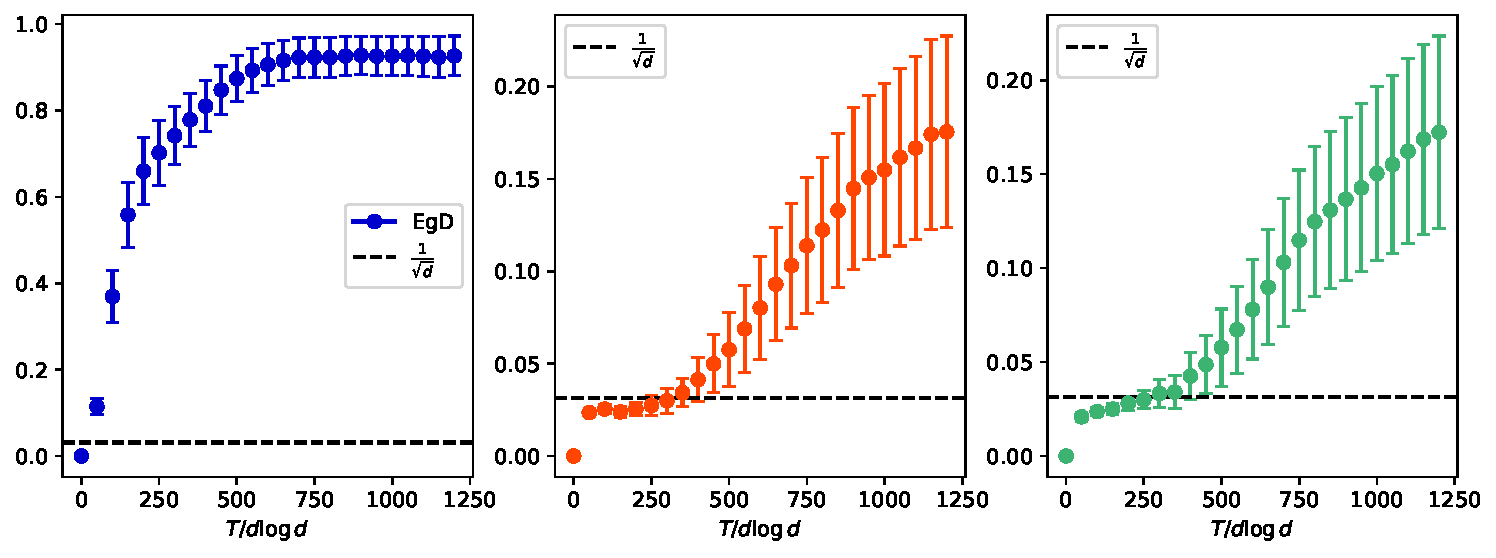
\includegraphics[width=0.75\linewidth]{figs/figs_SQStairH4_long}
    \caption{\textbf{Hierarchical learning --} Evolution of the maximum Cosine Similarities attained by EgD with different target directions $\{\vec w^\star_r\}_{r \in [k]}$ are identified by different colors: $\vec w^\star_1$ (blue), $\vec w^\star_2$ (orange), $\vec w^\star_3$ (green) as a function of the normalized iteration time. The target function is $f^\star_{\mathrm{sq-stair}}(\vec z)= \mathrm{He}_4(z_1) + \mathrm{sign}(z_1z_2z_3)$, that is an SQ-staircase (or grand staircase), not a CSQ-staircase. EgD learn $\vec w^\star_1$ in \(O(d\log d)\) steps and use the information to learn the other two directions in another \(O(d\log d)\) steps. SGD (not showed in the plot) cannot take advantage of the staircase mechanism since $\mathrm{He}_4(z_1)$ and $\mathrm{sign}(z_1z_2z_3)$ have information exponent \(\ell = 4\) and \(\ell = 3\) respectively. (See App.~\ref{2405:sec:app:implementation}).}   
    \label{2405:fig:main:staircase2}
\end{figure}
The Left panel in Fig.~\ref{2405:fig:main:staircase1} shows an example of the so-called staircase functions \citep{abbe2021staircase}, i.e. $f^\star(\vec z) = z_1 + z_1 \mathrm{He}_3(z_2)$. While one-pass SGD needs to learn hierarchically first the direction $\vec w^\star_1$ in $T=O(d)$ and then $\vec w^\star_2$ in $T=O(d^2)$, Algorithm~\ref{2405:algo:optimizer_main_step} easily learns both in linear time. This observation could lead to infer that hierarchical learning mechanisms are not present when more realistic training scenarios are considered. 



To refute this, we illustrate in the right panel of Fig.~\ref{2405:fig:main:staircase1} a scenario that precisely exemplifies the presence of hierarchical mechanisms within Algorithm~\ref{2405:algo:optimizer_main_step}. We run this algorithm on two different target functions, $f_{\mathrm{sign}}^\star(\vec{z}) = \mathrm{sign}(z_1z_2z_3)$ and $f^\star_{\mathrm{stair}}(\vec z) = \mathrm{He}_2(z_1) + \mathrm{sign}(z_1z_2z_3)$. We show in App. \ref{2405:sec:app:proofs} that $3-$sparse parities of the form $\mathrm{sign}(z_1z_2z_3)$ are hard functions even for SGD with data repetition (Algorithm~\ref{2405:algo:optimizer_main_step}), and indeed they are not learned in (almost) linear time. On the other hand, for the function $f^\star_{\mathrm{stair}}$, our simulations predict that the first direction $\vec w^\star_1$ is learned in $T = O(d \log d)$ iterations (see the rightmost panel of Fig.~\ref{2405:fig:main:multi_index_complete}). However, once the direction $\vec w^\star_1$ is learned, it can be used to obtain order-one correlation with $\{\vec w^\star_2, \vec w^\star_3\}$ again in $T = O(d \log d)$ steps. While the latter example belongs to the class of ``CSQ'' staircase function depicted in \cite{abbe2021staircase}, novel ``SQ'' hierarchical mechanisms arise in our framework, such as for instance the function $f_{\mathrm{sq-stair}}^\star(\vec z) = \mathrm{He}_4(z_1) + \mathrm{sign}(z_1z_2z_3)$ (see Fig.~\ref{2405:fig:main:staircase2}). 

The staircase picture in terms of generative exponent was discussed for AMP-type algorithm in \cite{troiani2024fundamental}. Our study indicate that this new class (they called grand staircase) is not restricted to AMP: We anticipate that grand staircase functions can be efficiently learned by two-layer networks when data reusing is permitted, whereas only standard staircase ones emerge  under single-pass SGD. Additional recent results by \citep{joshi2024complexity}  align with this perspective. 


% \begin{figure}
%     \centering
%     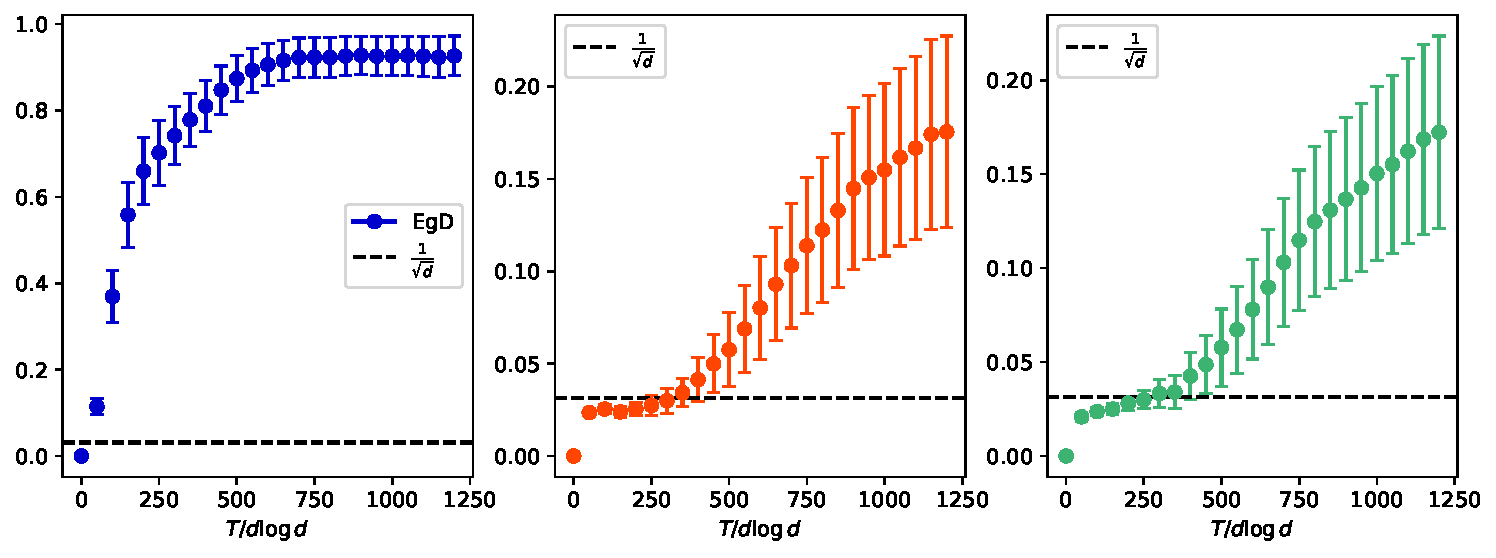
\includegraphics[width=.6\textwidth]{figs/figs_SQStairH4_long}
%     \caption{\textbf{Novel hierarchical picture of learning --} Evolution of the maximum Cosine Similarities attained by EgD with different target directions $\{\vec w^\star_r\}_{r \in [k]}$ are identified by different colors: $\vec w^\star_1$ (blue), $\vec w^\star_2$ (orange), $\vec w^\star_3$ (green) as a function of the normalized iteration time. The target function is $f^\star_{\mathrm{sq-stair}}(\vec z)= \mathrm{He}_4(z_1) + \mathrm{sign}(z_1z_2z_3)$, that is an SQ-staircase, but not a CSQ-staircase. EgD learn $\vec w^\star_1$ in \(O(d\log d)\) steps and use the information to learn the other two directions in another \(O(d\log d)\) steps. SGD (not showed in the plot) cannot take advantage of the staircas mechanism since $\mathrm{He}_4(z_1)$ and $\mathrm{sign}(z_1z_2z_3)$ have information exponent \(\ell = 4\) and \(\ell = 3\) respectively. See App.~\ref{2405:sec:app:implementation} for additional details.}
%     \label{2405:fig:main:staircase2}
    
% \end{figure}
